% !TeX root = main.tex
\chapter{Collaborative Manipulation}\label{ch:collaborative}
The contents of this chapter have been developed before the generalization of the vector field to Lie groups, thus it will lack the parlance of Lie groups. In the beginning, we will show how both works are related and how this chapter's vector field is a particular application of our generalization.
\section{Modelling and Problem Statement}
\begin{figure}[ht]
    \centering
    \def\svgwidth{.8\linewidth}
    \import{figures/}{collaborative_scheme.pdf_tex}
    \caption{Collaborative task}
    \label{fig:problem}
\end{figure}
The problem addressed in this section revolves around designing controller to guide a manipulated object along a predefined curve $\mathcal{C} \subset \mathbb{R}^3\times \text{SO}(3)$. The object's dynamics include uncertain parameters like mass and geometric properties. With $N$ agents involved in the manipulation process, a decentralized control law is devised for each agent. The agents are unaware of their precise positioning relative to a measurement point. It is assumed that each agent possesses the capability to measure the pose and velocity of the object's measurement point.

We consider the cooperative manipulation of a rigid body by a team of $N$ autonomous agents, as illustrated in \cref{fig:problem}. The body undergoes both translations and rotations. We establish two reference frames: the world-fixed inertial frame denoted $\mathfrak{I}$, and the body-fixed frame denoted $\mathfrak{B}$, centered at the body's center of mass, $\mathbf{b}\triangleq\mathbf{b}^\mathfrak{I}$. Additionally, a body-fixed measurement point, $\mathbf{p}^\mathfrak{B}$, is situated at a distance $\mathbf{r}_p^\mathfrak{B}$ from the body's center of mass.

The body possesses a mass $m$ and a constant inertia tensor $\mathbb{I}_\text{cm}^\mathfrak{B}$ about its center of mass. We assume each agent is rigidly attached to the body at $\mathbf{r}_i$ from $\mathbf{p}^\mathfrak{B}$. While $\mathbf{r}_i$ ideally should be expressed relative to a frame at $\mathbf{p}^\mathfrak{B}$, for simplicity, we interchangeably consider $\mathbf{r}_i= \mathbf{r}_i^\mathfrak{B}$. This assumption is made under the understanding that this information solely pertains to torque computations, and the frame associated with the measurement point shares the same orientation as that of the center of mass. Each agent exerts a wrench $\boldsymbol{\tau}_i$ onto the body.


Let $\mathbf{p}\triangleq\mathbf{p}^\mathfrak{I}(t)$ be the position of the measurement point in $\mathfrak{I}$ and let $\mathbf{R}\triangleq \mathbf{R}_\mathfrak{B}^\mathfrak{I}(t)$ be the rotation matrix from frame $\mathfrak{B}$ to frame $\mathfrak{I}$. Let the linear velocity of the point $\mathbf{p}$ expressed in frame $\mathfrak{I}$ be represented by $\dot{\mathbf{p}}$, and let $\boldsymbol{\omega}\triangleq\boldsymbol{\omega}^\mathfrak{I}(t)$ denote the angular velocity of frame $\mathfrak{B}$ with respect to $\mathfrak{I}$, expressed in $\mathfrak{I}$. Additionally, let $\ddot{\mathbf{p}}$ and $\dot{\boldsymbol{\omega}}$ represent the linear and angular accelerations of the body, respectively. Then, we can express the linear velocity at $\mathbf{p}$ as
\begin{align}
    \dot{\mathbf{p}} &= \frac{d}{dt}\bigl(\mathbf{b} + \mathbf{R}\mathbf{r}^\mathfrak{B}_p\bigr) 
    = \dot{\mathbf{b}} +\SL[\boldsymbol{\omega}]\mathbf{R}\mathbf{r}^\mathfrak{B}_p + \mathbf{R}\dot{\mathbf{r}}^\mathfrak{B} = \dot{\mathbf{b}} +\SL[\boldsymbol{\omega}]\mathbf{R}\mathbf{r}^\mathfrak{B}_p,
\end{align}
where the fact that $\mathbf{r}^\mathfrak{B}_p$ is constant in frame $\mathfrak{B}$ was used. The linear acceleration is given by
\begin{align}
    \ddot{\mathbf{p}} &= \frac{d}{dt}\bigl(\dot{\mathbf{b}} +\SL[\boldsymbol{\omega}]\mathbf{R}\mathbf{r}^\mathfrak{B}_p\bigr) 
    = \ddot{\mathbf{b}} + \SL[\dot{\boldsymbol{\omega}}]\mathbf{R}\mathbf{r}^\mathfrak{B}_p + \SL[\boldsymbol{\omega}]\SL[\boldsymbol{\omega}]\mathbf{R}\mathbf{r}^\mathfrak{B}_p.
\end{align}
Thus, the resulting force acting on the body is given by Newton's second law as
\begin{align}
    \mathbf{F}^\mathfrak{I}&=m\ddot{\mathbf{b}} = m\bigl(\ddot{\mathbf{p}} - \SL[\dot{\boldsymbol{\omega}}]\mathbf{R}\mathbf{r}^\mathfrak{B}_p - \SL[\boldsymbol{\omega}]\SL[\boldsymbol{\omega}]\mathbf{R}\mathbf{r}^\mathfrak{B}_p\bigr).
\end{align}
The total torque at point $\mathbf{p}$ expressed in the inertial frame is given by
\begin{align}
    \mathbf{T}^\mathfrak{I}_p = \mathbf{R}\mathbf{T}^\mathfrak{B}_p = \mathbf{R}\mathbb{I}^\mathfrak{B}_\text{cm}\mathbf{R}^T\dot{\boldsymbol{\omega}} + \SL[\boldsymbol{\omega}]\mathbf{R}\mathbb{I}^\mathfrak{B}_\text{cm}\mathbf{R}^T\boldsymbol{\omega} - \SL[\mathbf{R}\mathbf{r}^\mathfrak{B}_p]\mathbf{F}^\mathfrak{I}, \label{eq:torque-modelling}
\end{align}
expanding the last term, we have
\begin{align}
    - \SL[\mathbf{R}\mathbf{r}^\mathfrak{B}_p]\mathbf{F}^\mathfrak{I} = 
    - \SL[\mathbf{R}\mathbf{r}^\mathfrak{B}_p]\ddot{\mathbf{p}} - \SL[\mathbf{R}\mathbf{r}^\mathfrak{B}_p]\SL[\mathbf{R}\mathbf{r}_p^\mathfrak{B}]\dot{\boldsymbol{\omega}} + \SL[\mathbf{R}\mathbf{r}^\mathfrak{B}_p]\SL[\boldsymbol{\omega}]\SL[\boldsymbol{\omega}]\mathbf{R}\mathbf{r}_p^\mathfrak{B}. \label{eq:partial-torque1}
\end{align}
From Steiner's theorem \citep{lemos2018analytical}, we know that $\mathbb{I}^\mathfrak{B}_p = \mathbb{I}^\mathfrak{B}_\text{cm} - m\SL[\mathbf{r}_p^\mathfrak{B}]^2$, where $\mathbb{I}^\mathfrak{B}_p$ is the inertia tensor about point $\mathbf{p}$. Thus, we can obtain the following expression for the second term in \eqref{eq:partial-torque1}
\begin{align}
    - \SL[\mathbf{R}\mathbf{r}^\mathfrak{B}_p]\SL[\mathbf{R}\mathbf{r}_p^\mathfrak{B}]\dot{\boldsymbol{\omega}} = - \mathbf{R}\SL[\mathbf{r}^\mathfrak{B}_p]\mathbf{R}^T\mathbf{R}\SL[\mathbf{r}_p^\mathfrak{B}]\mathbf{R}^T\dot{\boldsymbol{\omega}} = \mathbf{R}\bigl(\mathbb{I}^\mathfrak{B}_p - \mathbb{I}^\mathfrak{B}_\text{cm}\bigr)\mathbf{R}^T\dot{\boldsymbol{\omega}}.
    \label{eq:partial-torque2}
\end{align}
Expanding the last term in \eqref{eq:partial-torque1}, we have
\begin{align}
    \begin{split}
        \SL[\mathbf{R}\mathbf{r}^\mathfrak{B}_p]\SL[\boldsymbol{\omega}]\SL[\boldsymbol{\omega}]\mathbf{R}\mathbf{r}_p^\mathfrak{B} &= \SL[\mathbf{R}\mathbf{r}^\mathfrak{B}_p]\SL[\boldsymbol{\omega}](\dot{\mathbf{p}} - \dot{\mathbf{b}})\\
        &= \SL[\mathbf{R}\mathbf{r}^\mathfrak{B}_p]\SL[\boldsymbol{\omega}]\dot{\mathbf{p}} - \SL[\mathbf{R}\mathbf{r}^\mathfrak{B}_p]\SL[\boldsymbol{\omega}]\dot{\mathbf{b}}.
    \end{split}
\end{align}
Applying Jacobi's identity, we obtain
\begin{align}
    % \begin{split}
    &m\SL[\SL[\dot{\mathbf{p}}]\mathbf{R}\mathbf{r}_p^\mathfrak{B}]\boldsymbol{\omega} + m\SL[\SL[\mathbf{R}\mathbf{r}_p^\mathfrak{B}]\boldsymbol{\omega}]\dot{\mathbf{p}}
    -m\SL[\SL[\dot{\mathbf{b}}]\mathbf{R}\mathbf{r}_p^\mathfrak{B}]\boldsymbol{\omega}  -m\SL[\SL[\mathbf{R}\mathbf{r}_p^\mathfrak{B}]\boldsymbol{\omega}]\dot{\mathbf{b}}\nonumber\\
    &=-m\SL[\SL[\mathbf{R}\mathbf{r}_p^\mathfrak{B}]\dot{\mathbf{p}}]\boldsymbol{\omega}  -m\SL[\SL[\boldsymbol{\omega}]\mathbf{R}\mathbf{r}_p^\mathfrak{B}]\dot{\mathbf{p}}
    -m\SL[\SL[\dot{\mathbf{b}}]\mathbf{R}\mathbf{r}_p^\mathfrak{B}]\boldsymbol{\omega}  +m\SL[\SL[\boldsymbol{\omega}]\mathbf{R}\mathbf{r}_p^\mathfrak{B}]\dot{\mathbf{b}}\nonumber\\
    &=-m\SL[\SL[\mathbf{R}\mathbf{r}_p^\mathfrak{B}]\dot{\mathbf{p}}]\boldsymbol{\omega}
    -m\SL[\dot{\mathbf{p}} - \dot{\mathbf{b}}]\dot{\mathbf{p}}
    -m\SL[\SL[\dot{\mathbf{b}}]\mathbf{R}\mathbf{r}_p^\mathfrak{B}]\boldsymbol{\omega}
    +m\SL[\dot{\mathbf{p}} - \dot{\mathbf{b}}]\dot{\mathbf{b}}\nonumber\\
    &=-m\SL[\SL[\mathbf{R}\mathbf{r}_p^\mathfrak{B}]\dot{\mathbf{p}}]\boldsymbol{\omega}
    +m\SL[\dot{\mathbf{b}}]\dot{\mathbf{p}}
    -m\SL[\SL[\dot{\mathbf{b}}]\mathbf{R}\mathbf{r}_p^\mathfrak{B}]\boldsymbol{\omega}
    +m\SL[\dot{\mathbf{p}}]\dot{\mathbf{b}}\nonumber\\
    &=-m\SL[\SL[\mathbf{R}\mathbf{r}_p^\mathfrak{B}]\dot{\mathbf{p}}]\boldsymbol{\omega}
    -m\SL[\SL[\dot{\mathbf{p}}-\SL[\boldsymbol{\omega}]\mathbf{R}\mathbf{r}_p^\mathfrak{B}]\mathbf{R}\mathbf{r}_p^\mathfrak{B}]\boldsymbol{\omega}\nonumber\\
    &=-m\SL[\SL[\mathbf{R}\mathbf{r}_p^\mathfrak{B}]\dot{\mathbf{p}}]\boldsymbol{\omega}
    -m\SL[\SL[\dot{\mathbf{p}}]\mathbf{R}\mathbf{r}_p^\mathfrak{B}]\boldsymbol{\omega}
    + m\SL[\SL[\SL[\boldsymbol{\omega}]\mathbf{R}\mathbf{r}_p^\mathfrak{B}]\mathbf{R}\mathbf{r}_p^\mathfrak{B}]\boldsymbol{\omega}\nonumber\\
    &=-m\SL[\SL[\mathbf{R}\mathbf{r}_p^\mathfrak{B}]\dot{\mathbf{p}}]\boldsymbol{\omega}
    -m\SL[\boldsymbol{\omega}]\SL[\mathbf{R}\mathbf{r}_p^\mathfrak{B}]\dot{\mathbf{p}}
    - m\SL[\boldsymbol{\omega}]\SL[\mathbf{R}\mathbf{r}_p^\mathfrak{B}]\SL[\mathbf{R}\mathbf{r}_p^\mathfrak{B}]\boldsymbol{\omega}\nonumber\\
    &=-m\SL[\SL[\mathbf{R}\mathbf{r}_p^\mathfrak{B}]\dot{\mathbf{p}}]\boldsymbol{\omega}
    -m\SL[\boldsymbol{\omega}]\SL[\mathbf{R}\mathbf{r}_p^\mathfrak{B}]\dot{\mathbf{p}}
    - m\SL[\boldsymbol{\omega}]\mathbf{R}\bigl(\mathbb{I}^\mathfrak{B}_p-\mathbb{I}^\mathfrak{B}_\text{cm}\bigr)\mathbf{R}^T\boldsymbol{\omega}. \label{eq:partial-torque3}
    % \end{split}
\end{align}
Finally, using \eqref{eq:torque-modelling}, \eqref{eq:partial-torque1}, \eqref{eq:partial-torque2}, and \eqref{eq:partial-torque3}, the resulting torque is expressed as
\begin{align}
    \mathbf{T}^\mathfrak{I}_p = &\mathbf{R}\mathbb{I}^\mathfrak{B}_\text{cm}\mathbf{R}^T\dot{\boldsymbol{\omega}} + \SL[\boldsymbol{\omega}]\mathbf{R}\mathbb{I}^\mathfrak{B}_\text{cm}\mathbf{R}^T\boldsymbol{\omega} - \SL[\mathbf{R}\mathbf{r}^\mathfrak{B}_p]\ddot{\mathbf{p}} + \mathbf{R}\bigl(\mathbb{I}^\mathfrak{B}_p - \mathbb{I}^\mathfrak{B}_\text{cm}\bigr)\mathbf{R}^T\dot{\boldsymbol{\omega}} \\
    &-m\SL[\SL[\mathbf{R}\mathbf{r}_p^\mathfrak{B}]\dot{\mathbf{p}}]\boldsymbol{\omega}
    -m\SL[\boldsymbol{\omega}]\SL[\mathbf{R}\mathbf{r}_p^\mathfrak{B}]\dot{\mathbf{p}}
    - m\SL[\boldsymbol{\omega}]\mathbf{R}\bigl(\mathbb{I}^\mathfrak{B}_p-\mathbb{I}^\mathfrak{B}_\text{cm}\bigr)\mathbf{R}^T\boldsymbol{\omega}\\
    = &\mathbf{R}\mathbb{I}^\mathfrak{B}_p\mathbf{R}^T\dot{\boldsymbol{\omega}} + \SL[\boldsymbol{\omega}]\mathbf{R}\mathbb{I}^\mathfrak{B}_p\mathbf{R}^T\boldsymbol{\omega} - \SL[\mathbf{R}\mathbf{r}^\mathfrak{B}_p]\ddot{\mathbf{p}} -m\SL[\SL[\mathbf{R}\mathbf{r}_p^\mathfrak{B}]\dot{\mathbf{p}}]\boldsymbol{\omega}\\
    &-m\SL[\boldsymbol{\omega}]\SL[\mathbf{R}\mathbf{r}_p^\mathfrak{B}]\dot{\mathbf{p}}
\end{align}

Define the pose $\mathbf{q} = (\mathbf{p}, \mathbf{R}) \in \mathbb{R}^3\times \text{SO}(3)$, and, abusing notation, let $\mathbb{R}^6\ni\dot{\mathbf{q}} = \left[\dot{\mathbf{p}}^T, \boldsymbol{\omega}^T \right]^T$ represent the system's linear and angular velocities. Additionally, let $\mathbb{R}^6\ni\ddot{\mathbf{q}} = \left[\ddot{\mathbf{p}}^T, \dot{\boldsymbol{\omega}}^T \right]^T$ represent the system's linear and angular accelerations.
With this notation, the dynamics can be succinctly expressed as
\begin{equation}
    \boldsymbol{\tau } = \mathbf {M}(\mathbf {q})\ddot{\mathbf {q}} + \mathbf {C}(\mathbf {q},\dot{\mathbf {q}})\dot{\mathbf {q}} + \mathbf{g}\label{eq:tau}
\end{equation}
where $\boldsymbol{\tau }$ denotes the total wrench applied to the body about the point $\mathbf{p}$. The system's Cartesian space mass matrix is represented by
\begin{equation}
    \mathbf {M}(\mathbf {q}) = \left[\begin{array}{cc}m\mathbf {I} & m\SL[\mathbf {R} \mathbf {r}_p^\mathfrak{B}] \\ -m\SL[\mathbf {R} \mathbf {r}_p^\mathfrak{B}] & \mathbf {R} \mathbb{I}^\mathfrak{B}_p \mathbf {R}^T \end{array} \right],\label{eq:Mcartesian}
\end{equation}
whereas the matrix $\mathbf {C}(\mathbf {q},\dot{\mathbf {q}})$ encompasses Coriolis and centrifugal terms:
\begin{equation}
\resizebox{0.88\columnwidth}{!}{$%
    \mathbf {C}(\mathbf {q},\dot{\mathbf {q}}) = \left[\begin{array}{cc}\boldsymbol{0}_{3\times3} & m\SL[\boldsymbol{\omega }] \SL[\mathbf {R} \mathbf {r}_p^\mathfrak{B}] \\ -m\SL[\boldsymbol{\omega }]\SL[\mathbf {R} \mathbf {r}_p^\mathfrak{B}] & \quad\SL[\boldsymbol{\omega }] \mathbf {R}\mathbb{I}_p^\mathfrak{B}\mathbf {R}^T 
    -m\SL[\SL[\mathbf {R}\mathbf {r}_p^\mathfrak{B}] \dot{\mathbf{p}}] \end{array} \right]. \label{eq:C}
$%
}
\end{equation}
The inertia tensor \(\mathbb{I}_p^\mathfrak{B}\) is determined by applying Steiner's theorem \citep{lemos2018analytical}: \(\mathbb{I}_p^\mathfrak{B} = \mathbb{I}_\text{cm}^\mathfrak{B} - m\SL[\mathbf{r}_p^\mathfrak{B}]^2\).

The dynamics described in \eqref{eq:tau} govern the motion of the body under the influence of the total wrench $\boldsymbol{\tau}$ applied about $\mathbf{p}$. This quantity needs to be expressed as a function of the wrenches $\boldsymbol{\tau}_i$ applied by each agent about their respective displacement $\mathbf{r}_i$ from $\mathbf{p}$. We represent $\boldsymbol{\tau}$ as the sum:
\begin{equation}
    \boldsymbol{\tau} = \sum_{i=1}^N\mathbf{G}(\mathbf{q}, \mathbf{r}_i)\boldsymbol{\tau}_i, \label{eq:tauNtauIrelation}
\end{equation}
where $\mathbf{G}$ denotes the grasp matrix, defined as:
\begin{equation}
    \mathbf{G}(\mathbf{q}, \mathbf{r}_i) = \begin{bmatrix}
        \mathbf{I}_{3\times3} & \mathbf{0}_{3\times3} \\
        \SL[\mathbf{R}\mathbf{r}_i] & \mathbf{I}_{3\times3} 
    \end{bmatrix}. \label{eq:graspmatrix}
\end{equation}

\section{Vector Field}
In this section, we use the vector field generalization to control a system in the Lie group $\mathbb{R}^3\times\text{SO}(3)$, described by the following first-order integrator model, where the control inputs are denoted as $\dot{\mathbf{p}}_d$ and $\boldsymbol{\omega}_d$:
\begin{align}
\begin{split}
    \dot{\mathbf{p}} &= \dot{\mathbf{p}}_d,\\
    \boldsymbol{\omega} &= \boldsymbol{\omega}_d.\label{eq:firstordersystemVF}
\end{split} 
\end{align}
Here $\mathbf{p}$ is the position, such that $\dot{\mathbf{p}}$ is the linear velocity, and $\boldsymbol{\omega}$ the angular velocity. 
The objective is to determine a vector field $\Psi:\mathbb{R}^3 \times \text{SO}(3)\to\mathbb{R}^6$, such that if the twist $\boldsymbol{\xi} = \bigl[\dot{\mathbf{p}}^\top\quad  \boldsymbol{\omega}^\top \bigr]^\top= \bigl[\dot{\mathbf{p}}_{d}^{\top}\quad \boldsymbol{\omega}_{d}^{\top} \bigr]^\top = \Psi$, the system \eqref{eq:firstordersystemVF} follows the target curve $\mathcal{C} \subset \mathbb{R}^3\times \text{SO}(3)$. Such a curve can be interpreted as a curve in Euclidean space with an orientation frame attached to each of its points, as shown in \cref{fig:curvewithframes}.
\begin{figure}[ht]
    \centering
    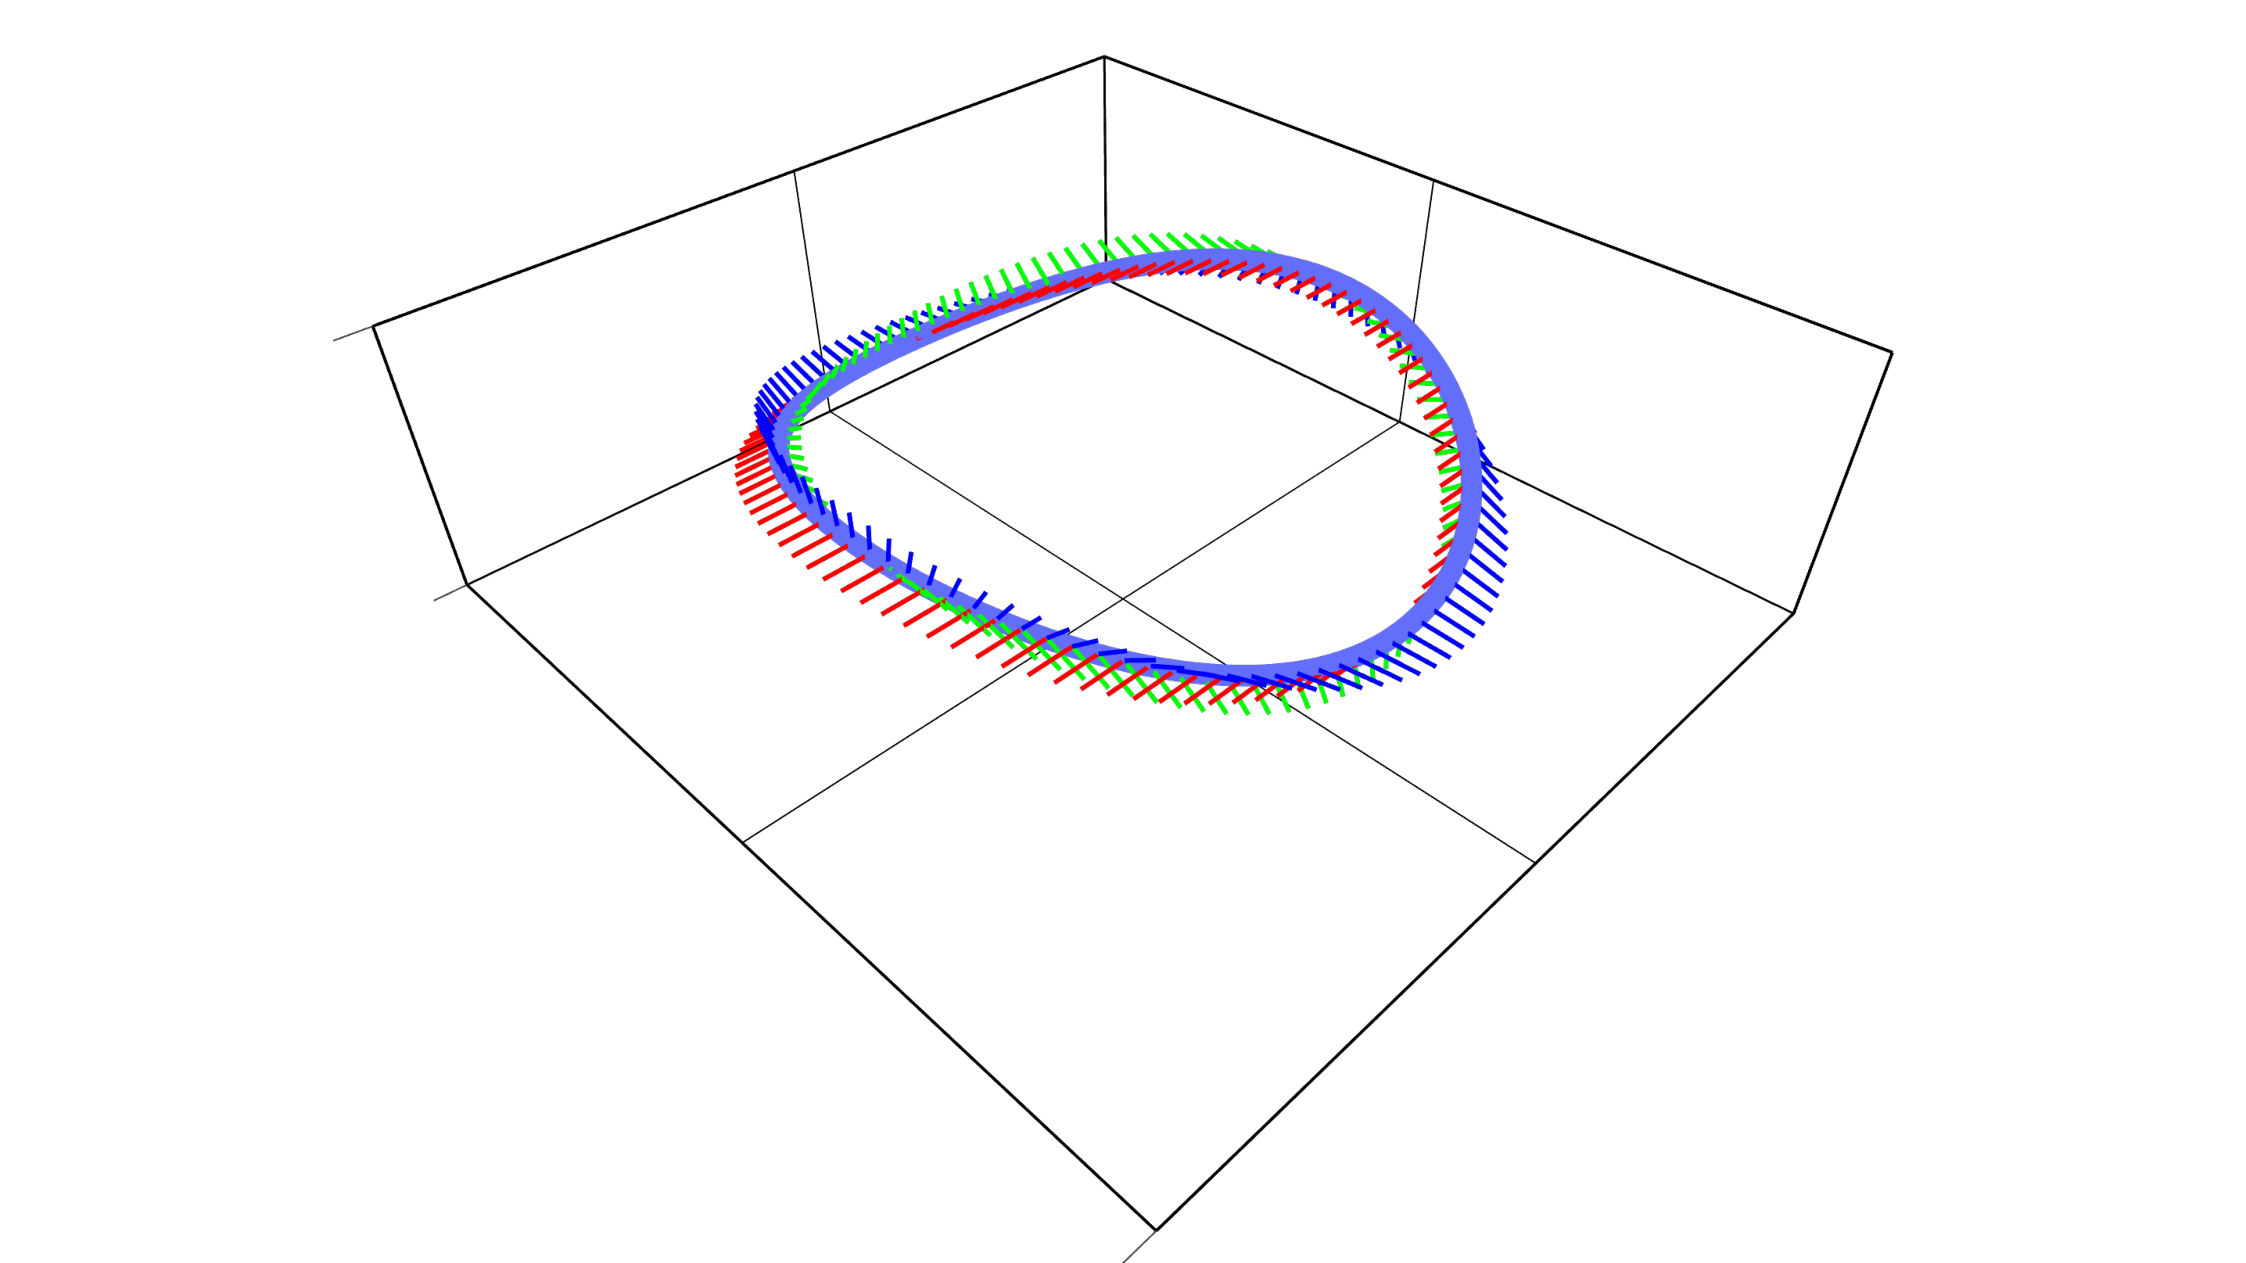
\includegraphics[width=.8\linewidth]{figures/curve_with_frames.pdf}
    \caption{Curve $\mathcal{C}$ in $\mathbb{R}^3\times\text{SO}(3)$. Orientation frames are depicted using RGB axes.}
    \label{fig:curvewithframes}
\end{figure}

In order to use our vector field methodology, we need to define an EE-distance function $\widehat{D}:\mathbb{R}^3\times\text{SO}(3)\times\mathbb{R}^3\times\text{SO}(3)\to\mathbb{R}_+$. For this, we will represent our system in $\text{ISE}(3)$ (see \cref{ex:independent-translation-rotation-ISE}). The EE-distance function $\widehat{D}: \text{ISE}(3) \times \text{ISE}(3) \to \mathbb{R}_+$ between two elements $\mathbf{V}, \mathbf{W}$ in the group $\text{ISE}(3)$ is defined as
\begin{align}
    \widehat{D}(\mathbf{V}, \mathbf{W}) = \| \log(\mathbf{V}^{-1}\mathbf{W}) \|_F.
\end{align}
Note that this is exactly the same distance as defined in \cref{ch:kinematic}, and so it possesses the same properties.
\begin{remark}
    In our original approach, we treat our system directly in $\mathbb{R}^3\times\text{SO}(3)$, and use the following distance function between two tuples:
    \begin{align}
        \widehat{D}(\mathbf{p}_1, \mathbf{R}_1, \mathbf{p}_2, \mathbf{R}_2) \equiv \frac{1}{2}\left(\|\mathbf{p}_1 - \mathbf{p}_2\|^2 + \beta\left\|\mathbf{I} - \mathbf{R}_2^{T}\mathbf{R}_1\right\|^2_F\right). \label{eq:cba-distance}
    \end{align}
    Although they are not equivalent, the change in the distance function will maintain consistency with our generalization to matrix Lie groups.
    
    Note that the distance in \eqref{eq:cba-distance} is left-invariant, and although it lacks a chainability proof, we can still show that the vector field it renders has a measure zero set of singularities. This change of distance is benefical, as it aligns with all the properties and proofs given.
\end{remark}

We will assume that the target curve $\mathcal{C}$ is twice diffenrentiable, closed, and without self-intersections. Thus, for an element $\mathbf{H}\in\text{ISE}(3)$ and a curve parametrization $\mathbf{H}_d(s)\in\text{ISE}(3)$, the vector field has the same expression
\begin{align}
    \Psi(\mathbf{H}) = k_N(\mathbf{H})\boldsymbol{\xi}_N(\mathbf{H}) + k_T(\mathbf{H})\boldsymbol{\xi}_T(\mathbf{H}),
\end{align}

% To begin, we define an error function $\widehat{D}\equiv\widehat{D}(\mathbf{p}, \mathbf{R}, \mathbf{p}_d, \mathbf{R}_d)$ that measures the discrepancy between a pose $(\mathbf{p}, \mathbf{R})$ and a desired pose $(\mathbf{p}_d, \mathbf{R}_d)$. The error function is expressed as follows
% \begin{equation}
%     \widehat{D}(\mathbf{p}, \mathbf{R}, \mathbf{p}_d, \mathbf{R}_d) \equiv \frac{1}{2}\left(\|\mathbf{p} - \mathbf{p}_d\|^2 + \beta\left\|\mathbf{I} - \mathbf{R}_d^{T}\mathbf{R}\right\|^2_F\right),\! \label{eq:errorfuncDtilde}
% \end{equation}
% where $\beta$ is a scaling parameter in squared meters utilized to maintain dimensional consistency. The Frobenius norm measures the parallelism of the rotation matrices columns, allowing parameter $\beta$ to balance position and orientation errors.

\section{Collaborative Manipulation}

% \textbf{MUDAR O COMEÇO, ESTA DEPENDENTE DA SECAO QUE VEM DEPOIS}
The problem addressed in this section revolves around designing an adaptive controller to guide a manipulated object along a predefined curve $\mathcal{C} \subset \mathbb{R}^3\times \text{SO}(3)$. The object's dynamics include uncertain parameters like mass and geometric properties. With $N$ agents involved in the manipulation process, a decentralized control law is devised for each agent. The agents are unaware of their precise positioning relative to the measurement point. It is assumed that each agent possesses the capability to measure the pose and velocity of the object's measurement point.
% The problem addressed in this work revolves around designing an adaptive controller to guide a manipulated object along a predefined curve. The dynamics of the object, expressed by equations \eqref{eq:tau} and \eqref{eq:tauNtauIrelation}, incorporate uncertain parameters such as mass properties $m$ and $\mathbb{I}_p^\mathfrak{B}$, as well as geometric properties $\mathbf{r}_p^\mathfrak{B}$ and $\mathbf{r}_i$. With $N$ agents involved in the manipulation process, a decentralized control law is devised for each agent. It is assumed that each agent possesses the capability to measure the pose and velocity of the object's measurement point.
% The curve $\mathcal{C} \subset \mathbb{R}^3\times \text{SO}(3)$ incorporates an orientation frame attached to each of its points, represented by a rotation matrix.
\vspace{-1mm}
\subsection{Decentralized Adaptive Control}
\vspace{-1mm}

In this section, we modify the adaptive control strategy proposed by \cite{Culbertson2021}. In their approach, an error vector is established between the system velocity and a velocity reference, resulting in a non-autonomous system. In contrast, our method defines the velocity error $\boldsymbol{\zeta}$ with respect to the vector field, thereby establishing an autonomous system. The vector is designed in such a way that when $\boldsymbol{\zeta}=0$, the system converges almost globally asymptotically to the curve $\mathcal{C}$. After this modification, the subsequent analysis proceeds similarly to the original approach. This error vector is expressed as:
% We define a velocity error vector $\mathbf{e}$ between the system velocities and the vector field. The vector is designed in such a way that when $\mathbf{e}=0$, the system converges almost globally asymptotically to and follows the curve $\mathcal{C}$. 
% The proposed adaptive control strategy draws inspiration from \cite{Culbertson2021} and aims to achieve similar outcomes using vector fields. We commence by defining an error vector $\mathbf{s}$ such that when $\mathbf{s}=0$, the system converges almost globally asymptotically to and follows the curve $\mathcal{C}$. This error vector is expressed as:
\begin{equation}
    \boldsymbol{\zeta} = \dot{\mathbf{q}} - \Psi,\label{eq:errorvector-s}
\end{equation}
where $\mathbf{q}$ denotes the pose of the measurement point, and $\dot{\mathbf{q}}$ represents its corresponding twist.

It's noteworthy that when $\boldsymbol{\zeta}=0$, the system follows the same integrator model \eqref{eq:firstordersystemVF}, with the vector field $\Psi$ acting as its input. Therefore, leveraging the insights from the previous section, we anticipate that the system will exhibit the desired behavior.

Moving forward, we introduce a reference model. Given that the system is overactuated (meaning multiple sets of control inputs $\boldsymbol{\tau}_i$ produce identical object dynamics), each agent can contribute a portion of the control effort. Thus, we define a set of $N$ positive constants $\alpha_i$, ensuring $\sum_{i=1}^N\alpha_i=1$. The reference model is then characterized by:
\begin{equation}
    \alpha _i \left(\mathbf {M}(\mathbf {q})\dot{\Psi} + \mathbf {C}(\mathbf {q},\dot{\mathbf {q}})\Psi + \mathbf {g} \right) = \boldsymbol{\tau}_i.
\end{equation}
Note that $\dot{\Psi}$ can be numerically approximated. Furthermore, exploiting the linearity in the parameters within the equations of motion \citep{spong2020robot}, we can represent the object's dynamics using a regressor matrix $\mathbf{Y}_o$ and a parameter vector $\mathbf{o}_i$. Here, $\mathbf{o}_i = \alpha_i\mathbf{o}$ denotes a vector of the object's physical parameters, $\mathbf{o}$, such as mass or moments of inertia, scaled by $\alpha_i$:
\begin{equation}
    \alpha _i \left(\mathbf {M}(\mathbf {q})\dot{\Psi} + \mathbf {C}(\mathbf {q},\dot{\mathbf {q}})\Psi + \mathbf {g} \right) = \mathbf {Y}_o\left(\mathbf{q},\dot{\mathbf{q}},\Psi, \dot{\Psi}\right) \mathbf {o}_i. \label{eq:linearparametrizationModelRef}
\end{equation}
Summing both sides of the equation from 1 to N yields the same dynamics as in equation \eqref{eq:tau} with an additional gravity term. Furthermore, since the agents estimate the scaled vector $\mathbf{o}_i$, the constants $\alpha_i$ need not be known a priori.

Next, we propose the following control law
\begin{equation}
    \boldsymbol{\tau}_i = \mathbf{G}(\hat{\mathbf{r}}_i)^{-1}\boldsymbol{\eta}_i,\label{eq:controlLawTaui}
\end{equation}
where $\hat{\mathbf{r}}_i$ represents the estimate of agent $i$'s displacement with respect to the measurement point, and
\begin{equation}
    \boldsymbol{\eta}_i = \mathbf{Y}_o\hat{\mathbf{o}}_i - \mathbf{K}_D\boldsymbol{\zeta}, \label{eq:controlLawEtai}
\end{equation}
with $\mathbf{K}_D$ being a positive definite matrix.

It is essential to note that:
\begin{equation}
    \mathbf{G}_i\mathbf{G}(\hat{\mathbf{r}}_i)^{-1} = \mathbf{I} - \mathbf{G}(\widetilde{\mathbf{r}}_i), \label{eq:relationGiGiInvtoProof}
\end{equation}
where $\widetilde{\mathbf{r}}_i = \hat{\mathbf{r}}_i - \mathbf{r}_i$.

Furthermore, we define the following linear parametrization:
\begin{equation}
    -\mathbf{G}(\widetilde{\mathbf{r}}_i)\boldsymbol{\eta}_i = \mathbf{Y}_r\left(\boldsymbol{\eta}_i, \mathbf{q}\right)\widetilde{\mathbf{r}}_i. \label{eq:linearParametrizationYrforEta}
\end{equation}
Using the provided expressions, we propose the following adaptation laws
\begin{align}
    \dot{\hat{\mathbf{o}}}_i &= -\boldsymbol{\Gamma}_o\mathbf{Y}^T_o\left(\mathbf{q},\dot{\mathbf{q}},\Psi, \dot{\Psi}\right)\boldsymbol{\zeta},  \label{eq:adaptiveOhat}\\
    \dot{\hat{\mathbf{r}}}_i &= -\boldsymbol{\Gamma}_r\mathbf{Y}^T_r\left(\boldsymbol{\eta}_i, \mathbf{q}\right)\boldsymbol{\zeta},  \label{eq:adaptiveRhat}
\end{align}
where $\hat{\mathbf{o}}_i$ represents agent $i$'s estimate of the system parameters. $\boldsymbol{\Gamma}_o$ and $\boldsymbol{\Gamma}_r$ are definite positive matrices corresponding to the adaptation gains.
\begin{theorem}
    Consider the control laws \eqref{eq:controlLawTaui} and \eqref{eq:controlLawEtai}, and the adaptation laws \eqref{eq:adaptiveOhat} and \eqref{eq:adaptiveRhat}. Under the proposed adaptive controller, all control signals remain bounded, and the system converges to and follows the curve $\mathcal{C}$ from almost all initial conditions.
\end{theorem}
\begin{proof}
    Consider the following Lyapunov function candidate
    \begin{equation}
        V = \frac{1}{2}\left( \boldsymbol{\zeta}^T \mathbf {M} \boldsymbol{\zeta} + \sum _{i=1}^{N} \widetilde{\mathbf{o}}_i^{\,T} \boldsymbol{\Gamma }_o^{-1}\widetilde{\mathbf{o}}_i + \widetilde{\mathbf{r}}_i^{\,T} \boldsymbol{\Gamma }_r^{-1} \widetilde{\mathbf{r}}_i \right),
    \end{equation}
    where $\widetilde{\mathbf {o}}_i = \hat{\mathbf{o}}_i - \mathbf{o}_i$ represents the parameter estimation error for agent $i$.

    Since the true parameters do not vary in time, i.e. $\dot{\widetilde{\mathbf {o}}}_i = \dot{\hat{\mathbf{o}}}_i$ and $\dot{\widetilde{\mathbf {r}}}_i = \dot{\hat{\mathbf{r}}}_i$, the time derivative of the Lyapunov candidate yields
    \begin{equation}
        \dot{V} = \boldsymbol{\zeta}^T \mathbf{M} \dot{\boldsymbol{\zeta}} + \frac{1}{2} \boldsymbol{\zeta}^T \dot{\mathbf{M}} \boldsymbol{\zeta} + \sum\limits_{i=1}^{N} \widetilde{\mathbf{o}}_i^{\,T} \boldsymbol{\Gamma}_o^{-1} \dot{\hat{\mathbf{o}}}_i + \widetilde{\mathbf{r}}_i^{\,T} \boldsymbol{\Gamma}_r^{-1}\dot{\hat{\mathbf{r}}}_i.
    \end{equation}
    Using the fact that $\dot{\boldsymbol{\zeta}} = \ddot{\mathbf{q}} - \dot{\Psi}$ and $\dot{\mathbf{q}} = \boldsymbol{\zeta} + \Psi$, along with the system dynamics equations, we can expand the term
    \begin{align} 
    \begin{split}
        \boldsymbol{\zeta}^T \mathbf {M} \dot{\boldsymbol{\zeta}} &= \boldsymbol{\zeta}^T\mathbf{M}(\ddot{\mathbf{q}} - \dot{\Psi})\\ 
        &= \boldsymbol{\zeta}^T\left(\textstyle \sum\limits_{i=1}^{N} \mathbf{G}_i\boldsymbol{\tau }_i - \mathbf{C}\Psi - \mathbf{C} \boldsymbol{\zeta} - \mathbf{g} - \mathbf{M}\dot{\Psi}\right).
    \end{split}
    \end{align} 
    Thus, using \eqref{eq:linearparametrizationModelRef}, \eqref{eq:controlLawTaui}, \eqref{eq:relationGiGiInvtoProof} and \eqref{eq:linearParametrizationYrforEta}, we find
    \begin{align}
    \begin{split}
        \dot{V} &= \sum\limits_{i=1}^{N} \boldsymbol{\zeta}^T\left(\boldsymbol{\eta}_i + \mathbf {Y}_r \widetilde{\mathbf {r}}_i - \mathbf {Y}_o \mathbf {o}_i\right) + \frac{1}{2}\boldsymbol{\zeta}^T\left(\dot{\mathbf {M}}-2\mathbf {C}\right)\boldsymbol{\zeta} \!\\ &\quad \quad + \widetilde{\mathbf {o}}_i^{\,T} \boldsymbol{\Gamma }_o^{-1} \dot{\hat{\mathbf {o}}}_i + \widetilde{\mathbf {r}}_i^{\,T} \boldsymbol{\Gamma }_r^{-1}\dot{\hat{\mathbf {r}}}_i. 
        \end{split}
    \end{align}
    Noting that $\dot{\mathbf{M}} - 2\mathbf{C}$ is skew-symmetric, and applying \eqref{eq:controlLawEtai} while substituting adaptation laws \eqref{eq:adaptiveOhat} and \eqref{eq:adaptiveRhat}, we have:
    \begin{align}
       \hspace{-2mm} \dot{V} &{=} \sum\limits_{i=1}^{N} \boldsymbol{\zeta}^T\!\!\left({-}\mathbf{K}_D\boldsymbol{\zeta} {+} \mathbf {Y}_r \widetilde{\mathbf {r}}_i {+}\mathbf{Y}_o \widetilde{\mathbf{o}}_i\right)  {-} \widetilde{\mathbf {o}}_i^{\,T}\mathbf{Y}_o^T\boldsymbol{\zeta} {-} \widetilde{\mathbf {r}}_i^{\,T}\mathbf{Y}_r^T\boldsymbol{\zeta}. 
    \end{align}
    Note that all terms are scalars, hence we can transpose them, which results in
    \begin{equation}
        \dot{V} = -N\boldsymbol{\zeta}^T\mathbf{K}_D\boldsymbol{\zeta} \le 0.
    \end{equation}
    Thus, $\boldsymbol{\zeta}\to0$ as $t\to\infty$, and almost all trajectories converge asymptotically to $\mathcal{C}$. The curve circulation is ensured by the tangent component. 
    % To show this, we invoke Barbalat's Lemma \citep[p. 323]{khalil2002nonlinear} and prove that $\dot{V}$ is uniformly continuous. First, note that since $\dot{V}\le0$ and $V$ is lower bounded, this implies that $\mathbf{s}, \widetilde{\mathbf {o}}_i, \widetilde{\mathbf {r}}_i$ are bounded for all $i$. $\ddot{V}$ is given by:
    % % \begin{equation}
    %     \ddot{V} = -N\mathbf{s}^T\mathbf{K}_D\dot{\mathbf{s}}.
    % \end{equation}
    % Then, if $\dot{\mathbf{s}}$ is bounded, the proof is complete. Note that we can write the following
    % \begin{equation}
    %     \mathbf{M}\dot{\mathbf{s}} = \mathbf{M}(\ddot{\mathbf{q}} - \dot{\Psi}) = \sum_{i=1}^{N} (\mathbf{Y}_o \widetilde{\mathbf{o}}_i + \mathbf{Y}_r \widetilde{\mathbf{r}}_i) - (N\mathbf{K}_D + \mathbf{C})\mathbf{s}.
    % \end{equation}
    % The vector field and its derivative are inherently bounded due to their construction. Furthermore, as previously demonstrated, the remaining terms are also bounded. Given that $\mathbf{M}$ is definitively positive, its inverse $\mathbf{M}^{-1}$ exists, ensuring the boundedness of $\dot{\mathbf{s}}$.

    % This demonstrates that $\ddot{V}$ is bounded, implying that $\dot{V}$ is uniformly continuous, and consequently, $\mathbf{s}\to0$ as $t\to\infty$. Therefore, if the system does not initiate at the singularity where $\text{tr}\left(\mathbf{R}_d^{*T}\mathbf{R}\right)=-1$, then $\boldsymbol{\xi}-\Psi$ and $\mathbf{p}-\mathbf{p}^*$ approach zero, and $\mathbf{R}_d^{*T}\mathbf{R}$ tends to $\mathbf{I}$, ensuring the system's convergence to the curve $\mathcal{C}$. The system's trajectory follows the curve due to the tangent component.
\end{proof}